\documentclass[a4paper]{scrreprt}
\usepackage{fullpage} % Slightly more margins
\usepackage{amsfonts}
\usepackage[usenames,dvipsnames]{color}
\usepackage{fancyhdr}
\pagestyle{fancy}
\usepackage[english]{babel}
\selectlanguage{english}
\usepackage[utf8]{inputenc}
\usepackage{graphicx}
\usepackage{url}
\usepackage{textcomp}
\usepackage{amsmath}
\usepackage{lastpage}
\usepackage{pgf}
\usepackage{wrapfig}
\usepackage{fancyvrb}
\usepackage{listings} % Source code highlighting
\usepackage{algpseudocode} % Algorithms
\usepackage{courier}

\lstdefinelanguage{diff}{
  morecomment=[f][\color{blue}]{@@},     % group identifier
  morecomment=[f][\color{red}]-,         % deleted lines
  morecomment=[f][\color{OliveGreen}]+,       % added lines
  morecomment=[f][\color{NavyBlue}]{---}, % Diff header lines (must appear after +,-)
  morecomment=[f][\color{NavyBlue}]{+++},
}

% Create header and footer
\headheight 27pt
\pagestyle{fancyplain}
\lhead{\footnotesize{Object-Oriented Design, IV1350}}
\chead{}
\rhead{\footnotesize{Assignment 4 Report}}
\lfoot{}
\cfoot{\thepage (\pageref{LastPage})}

% Create title page
\title{Assignment 4}
\subtitle{Object-Oriented Design, IV1350}
\author{Emil Tullstedt emiltu@kth.se}
\date{2014-05-15}

\graphicspath{ {./images/} }
\lstset{basicstyle=\footnotesize\ttfamily, language=Java, numbers=left}

\begin{document}

\maketitle

\tableofcontents %Generates the TOC

\chapter{Introduction}

\begin{figure}[h]
  \begin{center}
    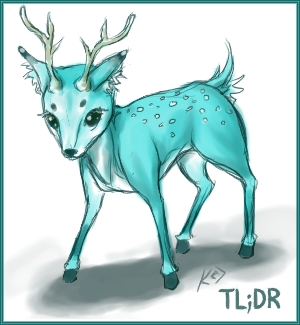
\includegraphics[scale=0.5]{tldr.jpg}
  \end{center}
\end{figure}

This report describes the process of implementing exceptions and GoF-patterns \texttt{Observer} and \texttt{Singleton} to a cache simulator made for a pre-graduate project in the course \textit{1350} at KTH in Stockholm. The implementation is not for production usage.

The report may be downloaded from \\\textbf{http://web.ict.kth.se/$\sim$emiltu/iv1350-emiltu-s4.pdf}

\begin{small}
While implementing the application, I co-operated with \textit{Martin Alge}, \textit{Jesper Falk} and \textit{Erik Pettersson}.
\end{small}

\chapter{Method}
\section{Design Patterns}
The theory behind design patterns is that there's a certain amount of abstract requirements that developers will face more often than others. When a requirement is often occurring for developers of a specific paradigm or language due to the nature of the applications that are built or the language itself, that requirement justifies a \textit{pattern}.

The \textit{pattern} is a tried way of solving a common issue that may be applied on different kinds of implementations, so the very same pattern that's applied to a rocket propellant system may also be used to program interactive Tamagochi-toys.

In object-oriented programming, due to the modular structure of the programming paradigm, patterns are quite commonly occurring and is thus part of any self-respecting object-orientational programmer's toolkit. During the mid 1990's, the book \textit{"Design Patterns: Elements of Reusable Object-Oriented Software"} was released by four authors, who subsequently became known as the \textit{Gang of Four}. The patterns they proposed is commonly referred to as GoF-patterns, and are widely-spread.

As per further developing the Cache Simulator implemented in \textit{Assignment 3}\footnote{http://web.ict.kth.se/$\sim$emiltu/iv1350-emiltu-s3.pdf} one of the requirements was to understand and implement design patterns. The application was already implementing the \textit{Singleton}-pattern in the \texttt{Storage}-class and an implementation of the \textit{Observer}-pattern was added to the \texttt{DataCache}-class and the \texttt{View}. The theory behind and the implementation of the patterns will be explained in the subsections \ref{subsec:Singleton} and \ref{subsec:Observer}.

\subsection{Storage as Singleton}
\label{subsec:Singleton}

The singleton is a pattern describing a class that describes a single object. The usage of the singleton is to find a middle-ground between a static class and a normal class. Implementing an enforcing singleton class is made by having a non-public constructor which is called when initializing a static variable containing the singleton itself. This variable may then be fetched by a static getter-method if you need to keep a good encapsulation.

For every advantage for using a singleton, there's quite often an equivalently strong disadvantage, such as singleton-classes quite often later are found being needed as normal classes, which can require a substantial rewrite of the application. There's also the issue of introducing a global state to the object oriented nature of the program, which by purist object oriented programmers is seen as a procedural programming plague.\footnote{See for example https://sites.google.com/site/steveyegge2/singleton-considered-stupid} Without arguing for or against the usage of singletons, it is widely used, and it's place in \textit{"Design Patterns"} by Gang of Four is hard to argue against.

When implementing the singleton (patch file is seen in it's entirety at \ref{subsec:storagepatch}) the nature of the assignment called for several design choices, primarily, the \texttt{Storage}'s construction isn't thread-safe or memory-efficient (it'll probably never be collected by the garbage collection). The implementation is shown in fig \ref{fig:diagstorage}.

\subsection{Observer Observing DataCache}
\label{subsec:Observer}

The \textit{observer} pattern attempts to solve the issue where an entity needs to track another entity for updates without having to constantly poll the other entity. The elegance of the \textit{observer} pattern is how it avoids causing a mess but still slightly sidestepping the notion that the \textit{models} never may communicate directly with the \textit{view}. The \textit{observer} uses a pre-defined interface (for reference, see \ref{subsec:datacacheobserver.java}) that defines how a view that wishes to be able to observe a observable object must implement a specific class.

Except for the slightly confusing concept of sidestepping the rules of \textit{MVC}, the observer-pattern also has the disadvantage that it's dependent on the observable object having access to call methods in the observing object and sometimes sending an unnecessary amount of data. Say for example a debugger which tracks memory, where polling might be a good idea to prevent a denial of service-attack caused by an overflow of updates being sent from the debugger when memory locations are changed. In this case, a second-wise poll may be an efficient solution. Another issue is that the observer pattern builds upon a mutually agreed upon API between anything that observes and the observed object, the creators of views must conform to a code style which they may not have agreed to. Whether this is an issue or not is a quite philosophic question.

The implementation of the \textit{observer} pattern in the cache simulator application is kept as simple as possible, where the \texttt{DataCache} (\ref{subsec:datacache.java}) stores a list of \texttt{DataCacheObserver}-implementors (\ref{subsec:datacacheobserver.java}) which are added and removed by a public function, which is also possibly being relayed through the \texttt{Controller} (\ref{subsec:controller.java}). The \texttt{View} is implemented as the observer, and is added to the list of observers on the user's request. Whenever the DataCache is updated (i.e. on misses when loading or storing data from it), the public function \texttt{recvDataCacheUpdates(String s)} is called with the content of the new cache to any observer. The implementation of the observer is shown in fig \ref{fig:diagobserver} and \ref{fig:interactobserver}.

\section{Exceptions}
The \texttt{AddressLayout} (\ref{subsec:addresslayout.java}) has added support for the new \texttt{IllegalAddressException} (\ref{subsec:illegaladdressexception.java}) which is thrown whenever the user enters an address which is not divisible by four (word length is defined in bytes). Adding the exception simultaneously caused for adding \texttt{throws} to the declaration of the \texttt{parseAddress()}-method in the \texttt{AddressLayout} and to the \texttt{executeInstruction()}-method in the \texttt{Instruction}-class (\ref{subsec:instruction.java}) and finally to the \texttt{executeInstruction()} in the \texttt{Controller} (\ref{subsec:controller.java}).

In order to catch the exception, the \texttt{View}-class is modified with a \texttt{try}-statement that catches the \texttt{IllegalAddressException} on which it prints the error that the \texttt{parseAddress()} includes with the exception as a description of the specific error and then continues by asking the user to enter another command.

\chapter{Result}
\label{sec:result}

\section{Controller and View}
\label{sec:sup}

\subsection{Class: Controller}
\label{subsec:controller.java}

The \texttt{Controller} has been updated to communicate adding and removing observers for the \texttt{DataCache} (\ref{subsec:datacache.java}) and handling \texttt{IllegalAddressLayout}. It also treats \texttt{Storage} (\ref{subsec:storage.java}) as a singleton-object correctly.

\lstinputlisting[language=Java]{cachesim/source/is/mjuk/cache/Controller.java}

\subsection{Class: View}
\label{subsec:view.java}

The \texttt{View} has been updated to act as an observer for \texttt{DataCache} (\ref{subsec:datacache.java})

\lstinputlisting[language=Java]{cachesim/source/is/mjuk/cache/View.java}

\section{Singleton}

\subsection{Class: Storage}
\label{subsec:storage.java}

The \texttt{Storage} was written as a \textit{singleton} from the very beginning and hasn't been changed since \textbf{Assignment 3}. Explanation of the implementation may be found in \ref{subsec:Singleton}.

\lstinputlisting[language=Java]{cachesim/source/is/mjuk/cache/Storage.java}

\section{Observer}

\subsection{Class: DataCache}
\label{subsec:datacache.java}

The \texttt{DataCache} is tested in \ref{subsec:datacachetest.java}.

\lstinputlisting[language=Java]{cachesim/source/is/mjuk/cache/DataCache.java}

\subsection{New Interface: DataCacheObserver}
\label{subsec:datacacheobserver.java}

\lstinputlisting[language=Java]{cachesim/source/is/mjuk/cache/DataCacheObserver.java}

\section{Exceptions}

\subsection{Class: AddressLayout}
\label{subsec:addresslayout.java}

\lstinputlisting[language=Java]{cachesim/source/is/mjuk/cache/AddressLayout.java}

\subsection{New Exception: IllegalAddressException}
\label{subsec:illegaladdressexception.java}

Exception-class for creating \texttt{IllegalAddressException}s for the \texttt{AddressLayout} when an address is unparseable.

\lstinputlisting[language=Java]{cachesim/source/is/mjuk/cache/IllegalAddressException.java}

\subsection{Class: Instruction}
\label{subsec:instruction.java}

\texttt{Instruction} has gotten a minor change to throw any \texttt{IllegalAddressException} that's thrown by \texttt{AddressLayout} (\ref{subsec:addresslayout.java}).

\lstinputlisting[language=Java]{cachesim/source/is/mjuk/cache/Instruction.java}

\section{Unchanged Files}
\label{sec:user}

These files have not been changed since assignment 3.

\subsection{Class: AddressDTO}
\label{subsec:addressdto.java}

\lstinputlisting[language=Java]{cachesim/source/is/mjuk/cache/AddressDTO.java}

\subsection{Class: Block}
\label{subsec:block.java}

\lstinputlisting[language=Java]{cachesim/source/is/mjuk/cache/Block.java}

\subsection{Class: CacheLayout}
\label{subsec:cachelayout.java}

\texttt{CacheLayout}'s comments has been changed minorly.

\lstinputlisting[language=Java]{cachesim/source/is/mjuk/cache/CacheLayout.java}

\subsection{Class: CacheSimulator}
\label{subsec:cachesimulator.java}

\lstinputlisting[language=Java]{cachesim/source/is/mjuk/cache/CacheSimulator.java}

\subsection{Class: InstructionDTO}
\label{subsec:instructiondto.java}

\lstinputlisting[language=Java]{cachesim/source/is/mjuk/cache/InstructionDTO.java}

\subsection{Enum: InstructionType}
\label{subsec:instructiontype.java}

\lstinputlisting[language=Java]{cachesim/source/is/mjuk/cache/InstructionType.java}

\subsection{Class: LayoutDTO}
\label{subsec:layoutdto.java}

\lstinputlisting[language=Java]{cachesim/source/is/mjuk/cache/LayoutDTO.java}

\subsection{Class: SimulationDTO}
\label{subsec:simulationdto.java}

\lstinputlisting[language=Java]{cachesim/source/is/mjuk/cache/SimulationDTO.java}

\subsection{Class: User}
\label{subsec:user.java}
\lstinputlisting[language=Java]{cachesim/source/is/mjuk/cache/User.java}

\section{Tests}

\subsection{New Class: AddressLayout Test}
\label{subsec:addresslayouttest.java}

The \texttt{AddressLayoutTest}-class is testing if the \texttt{AddressLayout} class can be created, parse a valid address and throw an exception on parsing an invalid address.

Test for the \texttt{AddressLayout}-class in \ref{subsec:addresslayout.java}.

\lstinputlisting[language=Java]{cachesim/test/is/mjuk/cache/AddressLayoutTest.java}

\subsection{Class: CacheLayout Test}
\label{subsec:cachelayouttest.java}

Updated to ensure to avoid \texttt{IllegalAddressException} (\ref{subsec:illegaladdressexception.java}).

Test for the \texttt{CacheLayout}-class in \ref{subsec:cachelayout.java}.

\lstinputlisting[language=Java]{cachesim/test/is/mjuk/cache/CacheLayoutTest.java}

\subsection{Class: DataCache Test}
\label{subsec:datacachetest.java}

Updated to ensure to avoid \texttt{IllegalAddressException} (\ref{subsec:illegaladdressexception.java}).

Test for the \texttt{DataCache}-class in \ref{subsec:datacachetest.java}.

\lstinputlisting[language=Java]{cachesim/test/is/mjuk/cache/DataCacheTest.java}

\subsection{Class: Storage Test}
\label{subsec:storagetest.java}

\footnotesize\textbf{Not updated since Assignment 3}\\
\normalsize Test for the \texttt{Storage}-class in \ref{subsec:storagetest.java}.

\lstinputlisting[language=Java]{cachesim/test/is/mjuk/cache/StorageTest.java}

\section{Sample Run}
\label{sec:samplerun}

\lstinputlisting[breaklines=true]{run4.txt}

\section{Patches}
These patches are the unchanged initial diffs for the git commit that introduced the running code. These do not necessarily represent the final state, which is accessible by reading the source files in it's entirety. Notably, the Javadoc-comments are not complete.

\subsection{Storage Patch}
\label{subsec:storagepatch}

\lstinputlisting[language=diff,breaklines=true]{diff/storage.diff}

\subsection{Exception Patch}
\label{subsec:exceptionpatch}

\lstinputlisting[language=diff,breaklines=true]{diff/exception.diff}


\subsection{Observer Patch}
\label{subsec:observerpatch}

\lstinputlisting[language=diff,breaklines=true]{diff/observer.diff}

\section{Utilities}

\subsection{Class: MisMath}
\label{subsec:mismath.java}
\lstinputlisting[language=Java]{cachesim/source/is/mjuk/utils/MisMath.java}

\chapter{Attachments}

\section{Diagrams}

\begin{figure}[h]
  \begin{center}
    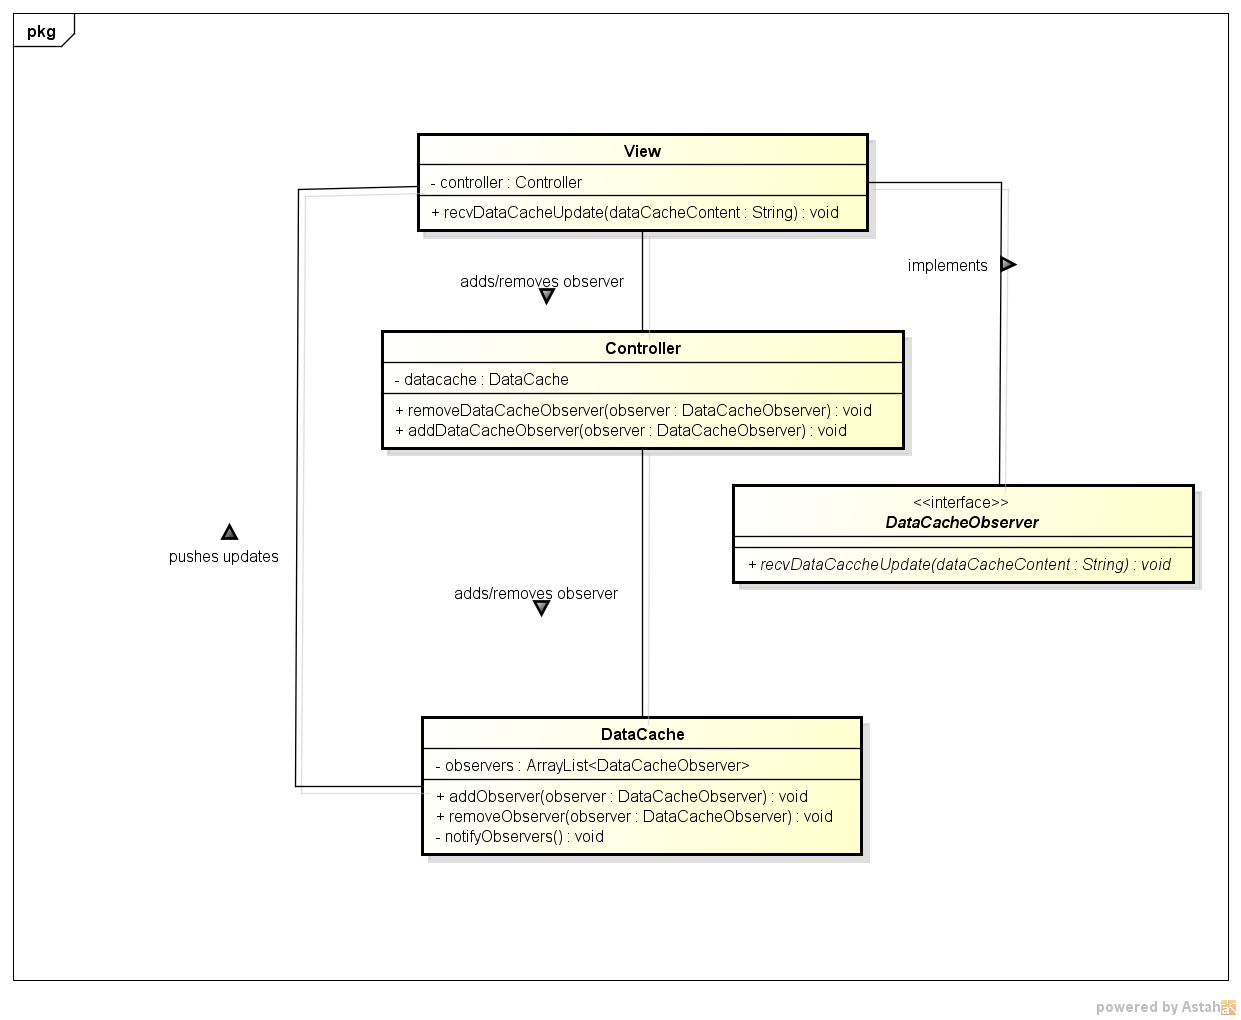
\includegraphics[scale=0.4]{ClassDiagramObserverPattern.png}
    \caption{Class Diagram for the implementation of the Observer Diagram}
    \label{fig:diagobserver}
  \end{center}
\end{figure}

\begin{figure}[h]
  \begin{center}
    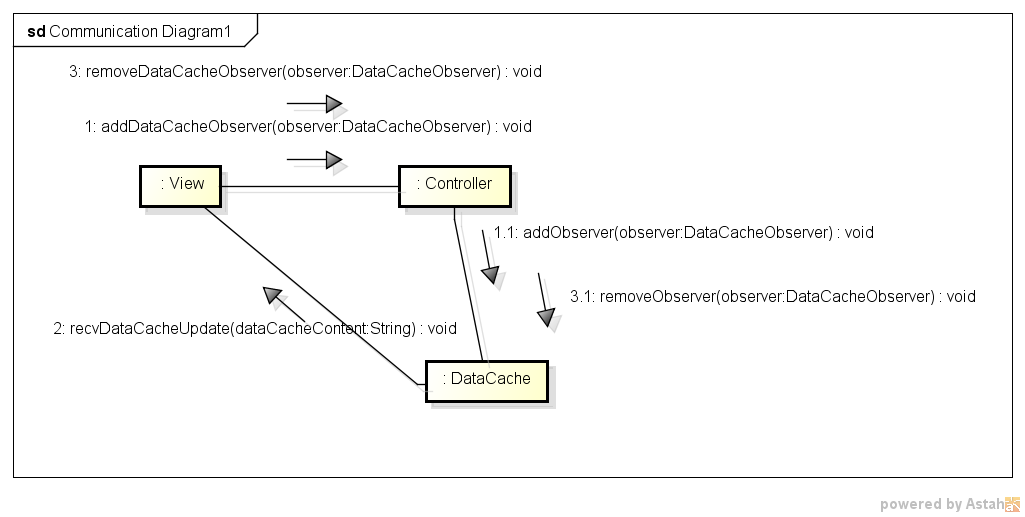
\includegraphics[scale=0.6]{ObserverInteractionDiagram.png}
    \caption{Interaction Diagram describing how the implementation of the \texttt{Observer}-pattern works}
    \label{fig:interactobserver}
  \end{center}
\end{figure}

\begin{figure}[h]
  \begin{center}
    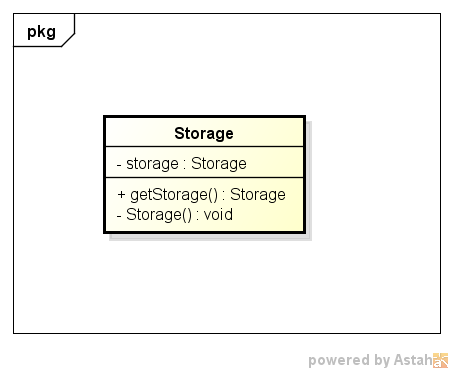
\includegraphics[scale=1.0]{ClassDiagramStorage.png}
    \caption{Class Diagram for the \texttt{Storage}-class, which implements the singleton pattern}
    \label{fig:diagstorage}
  \end{center}
\end{figure}

\end{document}
